\documentclass[serif, aspectratio=169]{beamer}
% \documentclass[serif]{beamer}  % for 4:3 ratio
\usepackage[T1]{fontenc} 
\usepackage{fourier} % see "http://faq.ktug.org/wiki/uploads/MathFonts.pdf" for other options
\usepackage{hyperref}
\usepackage{latexsym,amsmath,xcolor,multicol,booktabs,calligra}
\usepackage{graphicx,pstricks,listings,stackengine}
\usepackage{lipsum}

\author{Abdelhakim Zetati -- Lahcen Ezzara}
\title{Reinforcement Learning (RL)}
\subtitle{Tendances IT}
\institute{
   zetati.abdehakim@ensam-casa.ma -- ezzara.lahcen@ensam-casa.ma \\
    Université Hassan II de Casablanca \\
    ENSAM Casablanca \\
}
\date{\small Mercredi 18 Octobre 2024}
\usepackage{style}

% defs
\def\cmd#1{\texttt{\color{red}\footnotesize $\backslash$#1}}
\def\env#1{\texttt{\color{blue}\footnotesize #1}}
% set colors
\definecolor{hkustyellow}{RGB}{167, 131, 55}
\definecolor{hkustblue}{RGB}{0, 56, 116}
\definecolor{hkustred}{RGB}{209, 51, 59}


\lstset{
    basicstyle=\ttfamily\small,
    keywordstyle=\bfseries\color{deepblue},
    emphstyle=\ttfamily\color{deepred},    % Custom highlighting style
    stringstyle=\color{deepgreen},
    numbers=left,
    numberstyle=\small\color{halfgray},
    rulesepcolor=\color{red!20!green!20!blue!20},
    frame=shadowbox,
}

%- --- --- --- --- --- --- --- --- --- --- --- --- --- --- --- 
\begin{document}

\begin{frame}
    \titlepage
    \vspace*{-0.6cm}
    \begin{figure}[htpb]
        \begin{center}
            
\includegraphics[keepaspectratio, scale=0.15]{images/ensam-casa.png}
        \end{center}
    \end{figure}
\end{frame}

\begin{frame}    
\tableofcontents[sectionstyle=show,
subsectionstyle=show/shaded/hide,
subsubsectionstyle=show/shaded/hide]
\end{frame}

% Introduction au RL --- --- --- --- --- --- --- --- --- --- --- --- 

\section{Introduction au RL}

\begin{frame}{Comprendre l'apprentissage par renforcement}
	\frametitle<presentation>{Comprendre l'apprentissage par renforcement}
	
		\begin{itemize}
			\item \textbf{L'apprentissage par renforcement (RL)} se distingue en apprenant à travers des interactions avec un environnement pour maximiser une fonction de récompense, sans étiquettes correctes prédéfinies, ce qui le rend utile pour la prise de décision dans des environnements complexes.
		\end{itemize}

\end{frame}

% Interface Agent-Environnement --- --- --- --- --- --- --- --- --- --- --- ---

\section{Interface Agent-Environnement}

\begin{frame}{L'interface agent-environnement d'un système d'apprentissage par renforcement}
	\frametitle<presentation>{L'interface agent-environnement d'un système d'apprentissage par renforcement}
	
	L'état de l'agent est composé de ses variables, et il interagit avec l'environnement à travers des actions, recevant des récompenses qui guident ses transitions d'état. Le processus d'apprentissage implique de trouver un équilibre entre l'exploration (essayer de nouvelles actions) et l'exploitation (choisir des actions avec des récompenses connues) pour maximiser les récompenses cumulées au fil du temps. 
	
\end{frame}

\begin{frame}{L'interaction entre l'agent et son environnement}
	\frametitle<presentation>{L'interaction entre l'agent et son environnement}
	
	\begin{figure}[htpb]
		\centering
		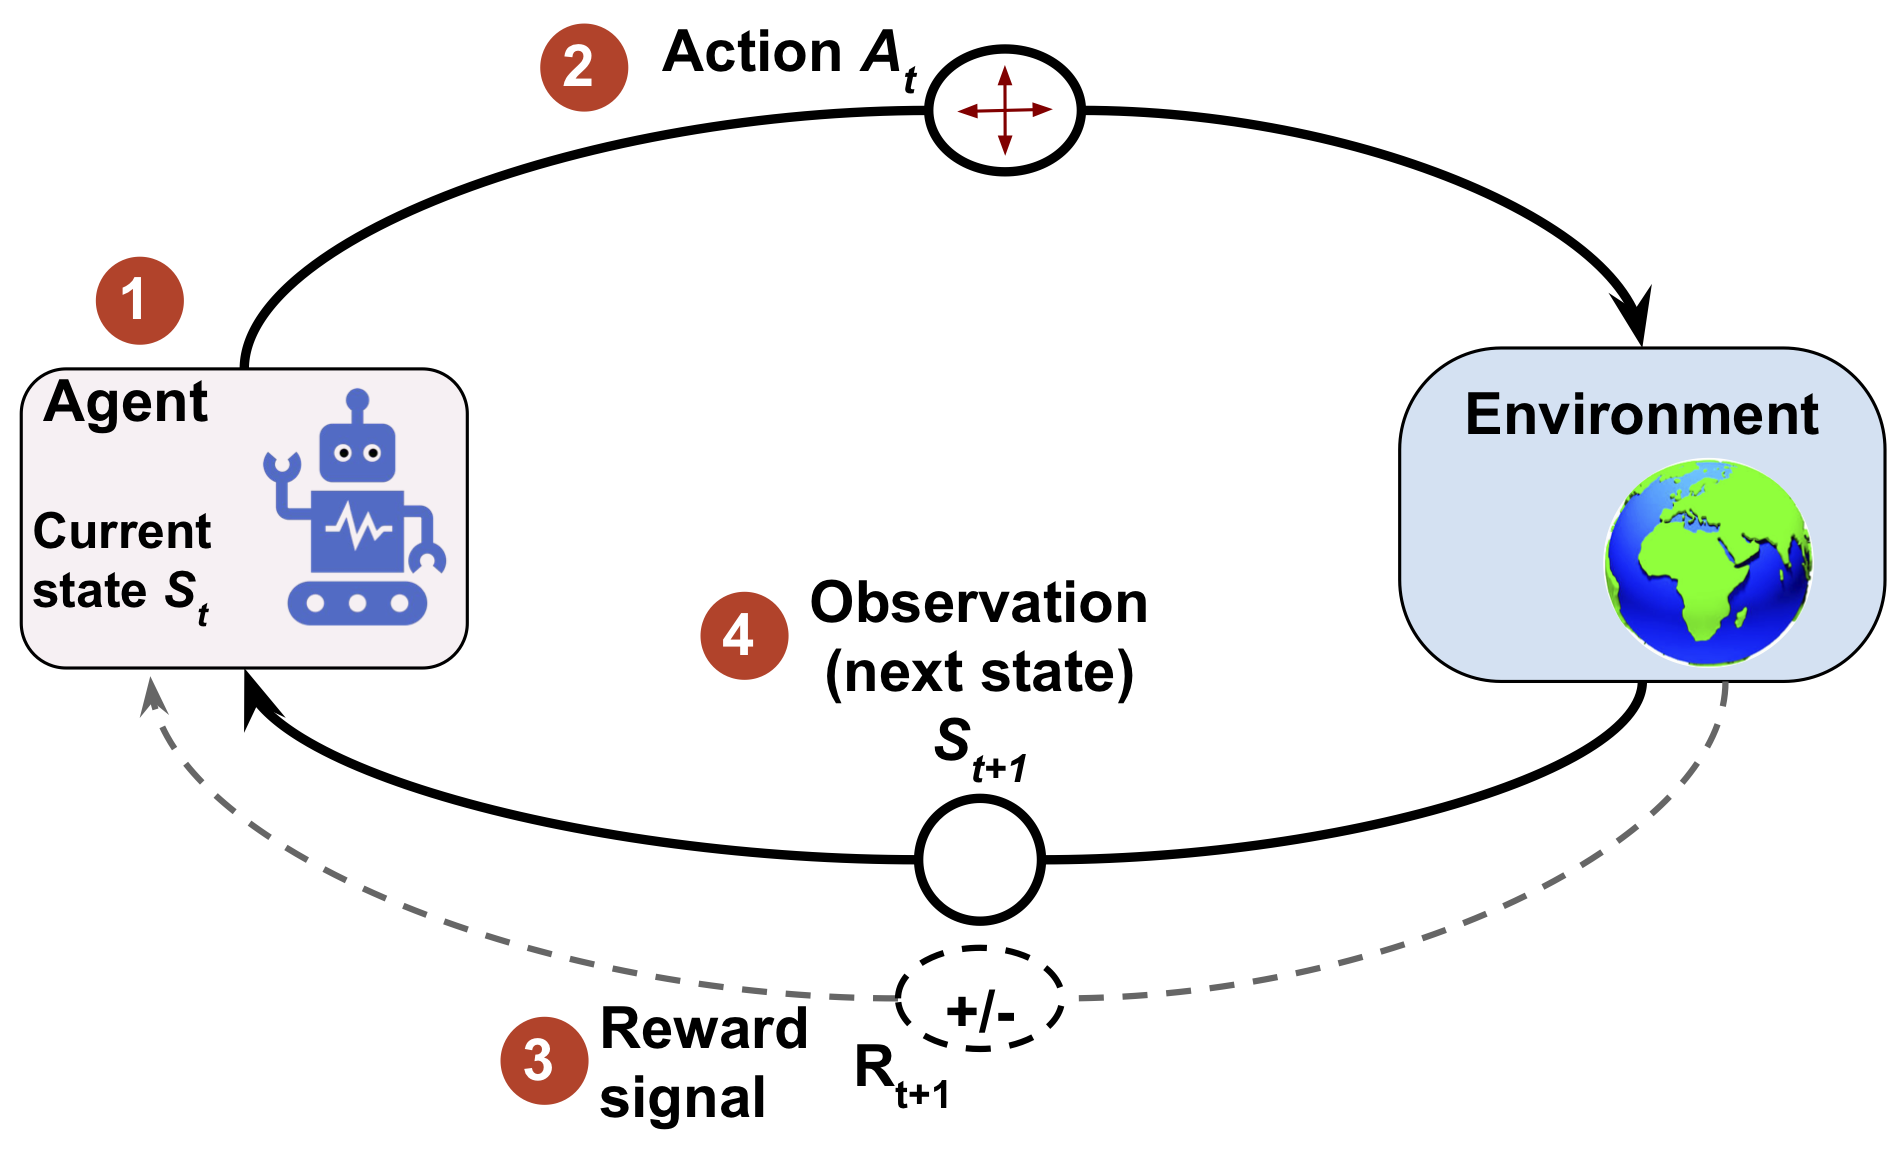
\includegraphics[keepaspectratio, scale=0.6]{images/interface-agent-environnement.png}
		\caption{L'interaction entre l'agent et son environnement}
	\end{figure}
	
\end{frame}


% Fondations Théoriques --- --- --- --- --- --- --- --- --- --- --- 
\section{Fondations Théoriques}

\begin{frame}{Les processus de décision de Markov}
	\frametitle<presentation>{Les processus de décision de Markov}
	
	En général, le type de problèmes que l'apprentissage par renforcement (RL) traite est généralement formulé comme des processus de décision de Markov (MDP). L'approche standard pour résoudre les problèmes MDP est d'utiliser la programmation dynamique, mais l'apprentissage par renforcement offre certains avantages clés par rapport à la programmation dynamique. 
	
\end{frame}

\begin{frame}{La formulation mathématique des processus de décision de Markov}
	\frametitle{La formulation mathématique des processus de décision de Markov}
	
	La distribution de probabilité pour \( S_{t+1} = s' \) et \( R_{t+1} = r \) peut être écrite comme une probabilité conditionnelle sur l'état précédent \( S_t \) et l'action prise \( A_t \) comme suit :
	
	\[
	p(s', r \mid s, a) \equiv P(S_{t+1} = s', R_{t+1} = r \mid S_t = s, A_t = a)
	\]
	
	\vspace{20pt}
	
	Deux approches principales pour traiter ce problème sont les méthodes Monte Carlo (MC) sans modèle et les méthodes de différence temporelle (TD). Le tableau suivant présente les deux principales catégories et les branches de chaque méthode :
	
\end{frame}

\begin{frame}{Les différents modèles à utiliser en fonction de la dynamique de l'environnement}
	\frametitle{Les différents modèles à utiliser en fonction de la dynamique de l'environnement}
	
	\begin{figure}[htpb]
		\centering
		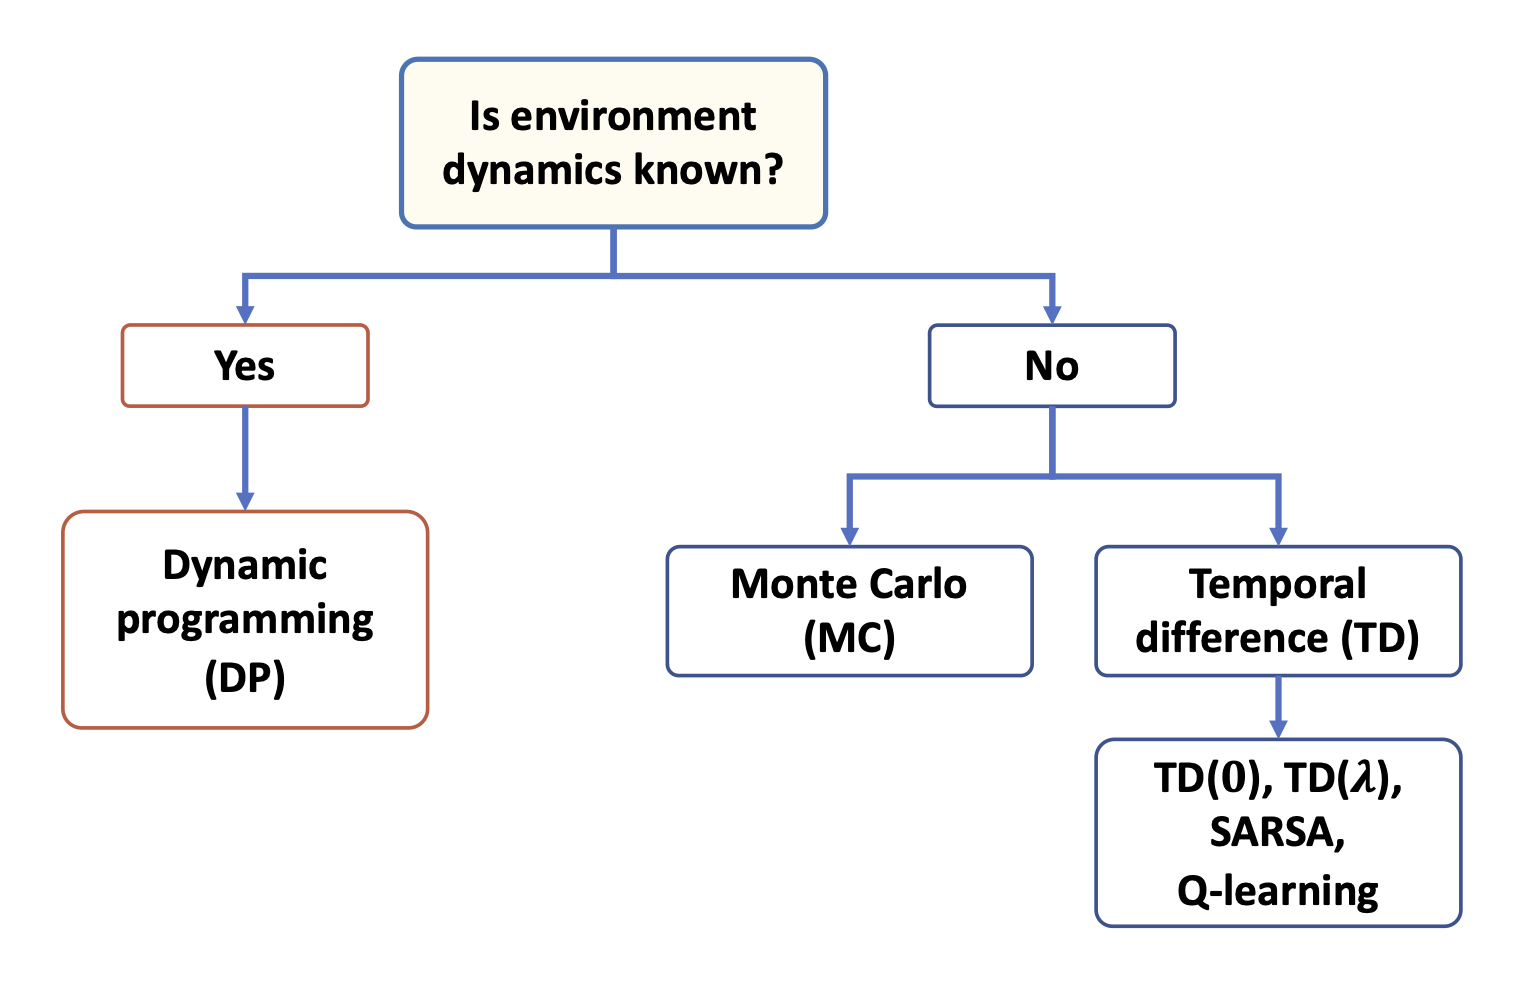
\includegraphics[keepaspectratio, scale=0.7]{images/markov.png}
		\caption{Les différents modèles à utiliser en fonction de la dynamique de l'environnement}
	\end{figure}
	
\end{frame}


\begin{frame}{Dynamique de l'environnement : déterministe ou stochastique}
	\frametitle{Dynamique de l'environnement : déterministe ou stochastique}
		
		La dynamique de l'environnement peut être considérée comme déterministe si des actions particulières pour des états donnés sont toujours ou jamais prises, c'est-à-dire \(p(s', r \mid s, a) \in \{0,1\}\). Sinon, dans le cas plus général, l'environnement aurait un comportement stochastique.
		
\end{frame}


% Terminologie du RL --- --- --- --- --- --- --- --- --- --- --- 
\section{Terminologie du RL}

\begin{frame}{Terminologie de l'apprentissage par renforcement}
	\frametitle{Terminologie de l'apprentissage par renforcement}
	
	En apprentissage par renforcement, plusieurs concepts doivent s'envisager pour comprendre comment un agent interagit avec son environnement et maximise une fonction de récompense.
	
	\vspace{10pt}
	
	\begin{itemize}
		\item \textbf{Retour (Return)}.
		
		\item \textbf{Politique (Policy)}.
		
		\item \textbf{Fonction de Valeur (Value Function)}.
	\end{itemize}
	
\end{frame}


\begin{frame}{Retour (Return)}
	\frametitle{Retour (Return)}
	
	Le retour au temps t en apprentissage par renforcement est la récompense cumulée totale d'un épisode, calculée comme suit :
	
	\[
	G_t \equiv R_{t+1} + \gamma R_{t+2} + \gamma^2 R_{t+3} + \cdots = \sum_{k=0} \gamma^k R_{t+k+1}
	\]
	
	\vspace{10pt}
	
	\[
	G_t = R_{t+1} + \gamma G_{t+1} = r + \gamma G_{t+1}
	\]
	
\end{frame}

\begin{frame}{Politique (Policy)}
	\frametitle{Politique (Policy)}
	
	Une politique, généralement notée \( \pi(a \mid s) \), est une fonction qui détermine la prochaine action à prendre. Elle peut être soit déterministe, soit stochastique (c'est-à-dire la probabilité de prendre la prochaine action). Une politique stochastique a alors une distribution de probabilité sur les actions qu'un agent peut prendre dans un état donné :
	
	\[
	\pi(a \mid s) \equiv P[A_t = a \mid S_t = s]
	\]
	
	\vspace{10pt}
	
	La politique optimale \( \pi_*(a \mid s) \) est celle qui génère le retour le plus élevé.
	
\end{frame}


\begin{frame}{Fonction de Valeur (Value Function)}
	\frametitle{Fonction de Valeur (Value Function)}
	
	La fonction de valeur, également appelée fonction de valeur d'état, mesure la qualité de chaque état, c'est-à-dire à quel point il est bon ou mauvais d'être dans un état particulier. Notez que le critère de qualité est basé sur le retour. Maintenant, sur la base du retour \( G_t \), nous définissons la fonction de valeur de l'état \( s \) comme le retour attendu (le retour moyen sur tous les épisodes possibles) après avoir suivi la politique \( \pi \) :
	
	\vspace{10pt}
	
	\[
	v_\pi(s) \equiv E_\pi[G_t \mid S_t = s] = E_\pi\left[\sum_{k=0} \gamma^{k+1} R_{t+k+1} \mid S_t = s\right]
	\]
	
\end{frame}


\begin{frame}{Fonction de Valeur (Value Function)}
	\frametitle{Fonction de Valeur (Value Function)}
	
	De plus, nous pouvons également définir une valeur pour chaque paire état-action, qui est appelée la fonction de valeur d'action et est notée \( q_\pi(s, a) \). La fonction de valeur d'action fait référence au retour attendu \( G_t \) lorsque l'agent est à l'état \( S_t = s \) et prend l'action \( A_t = a \). En étendant la définition de la fonction de valeur d'état aux paires état-action, nous obtenons ce qui suit :
	
	\[
	q_\pi(s, a) \equiv E_\pi[G_t \mid S_t = s, A_t = a] = E_\pi\left[\sum_{k=0} \gamma^{k+1} R_{t+k+1} \mid S_t = s, A_t = a\right]
	\]
	
	Ceci est similaire à la référence à la politique optimale en tant que \( \pi_*(a \mid s) \); \( v_*(s) \) et \( q_*(s, a) \) désignent également les fonctions de valeur d'état et de valeur d'action optimales.
	
\end{frame}

\begin{frame}{Quelle est la différence entre la récompense, le retour et la fonction de valeur?}
	\frametitle{Quelle est la différence entre la récompense, le retour et la fonction de valeur?}
	
	\begin{figure}[htpb]
		\centering
		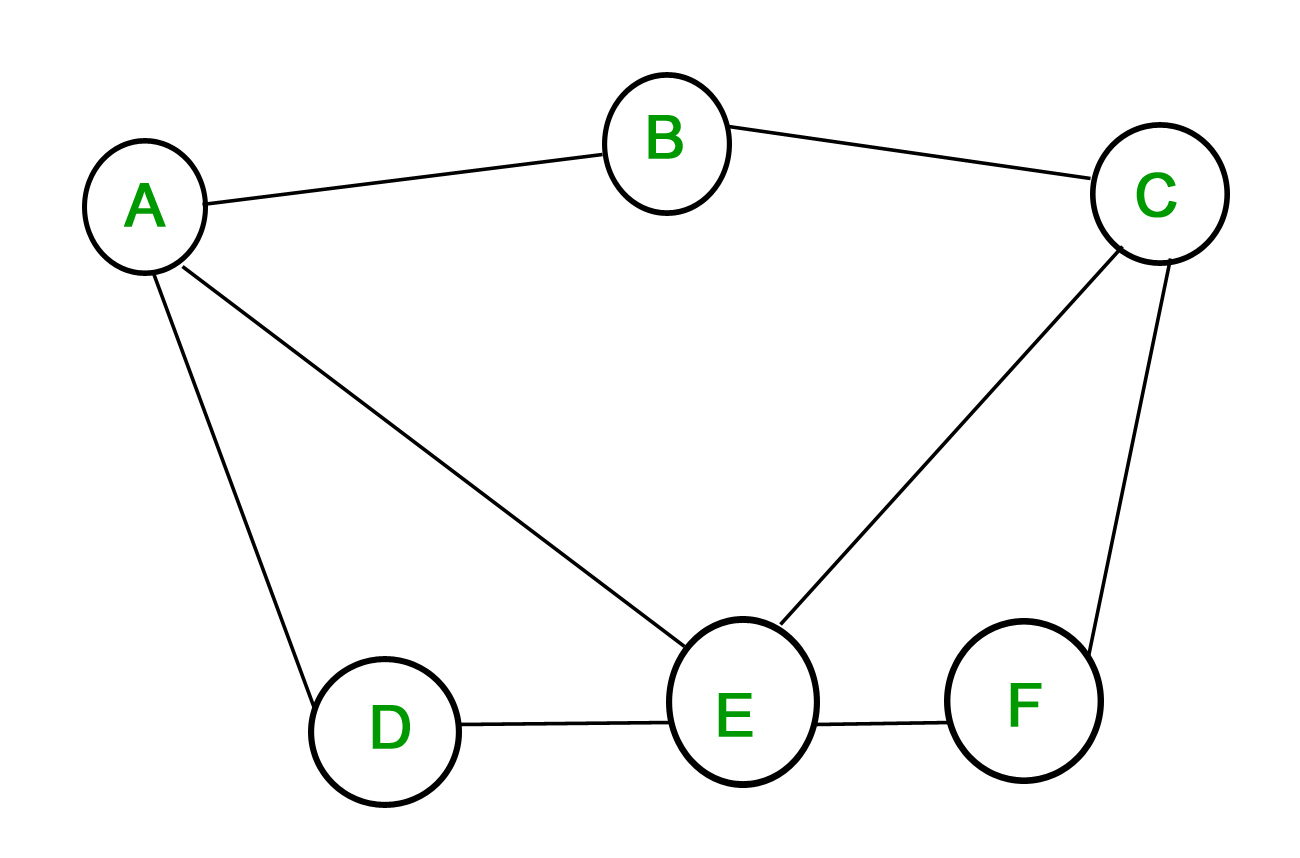
\includegraphics[keepaspectratio, scale=0.2]{images/graph.jpg}
		\caption{Graphe}
	\end{figure}
	
\end{frame}


% Deep Q-Learning --- --- --- --- --- --- --- --- --- --- --- 
\section{Deep Q-Learning}

\begin{frame}{Deep Q-Learning}
	\frametitle{Deep Q-Learning}
	
	Lorsque la fonction d'approximation, \( q_w(x_s, a) \), est un réseau de neurones profond (DNN), le modèle résultant est appelé un réseau Q profond (DQN). Pour entraîner un modèle DQN, les poids sont mis à jour conformément à l'algorithme Q-learning.
	
\end{frame}

\begin{frame}{Exemple de DQN}
	\frametitle{Exemple de DQN}
	
	\begin{figure}[htpb]
		\centering
		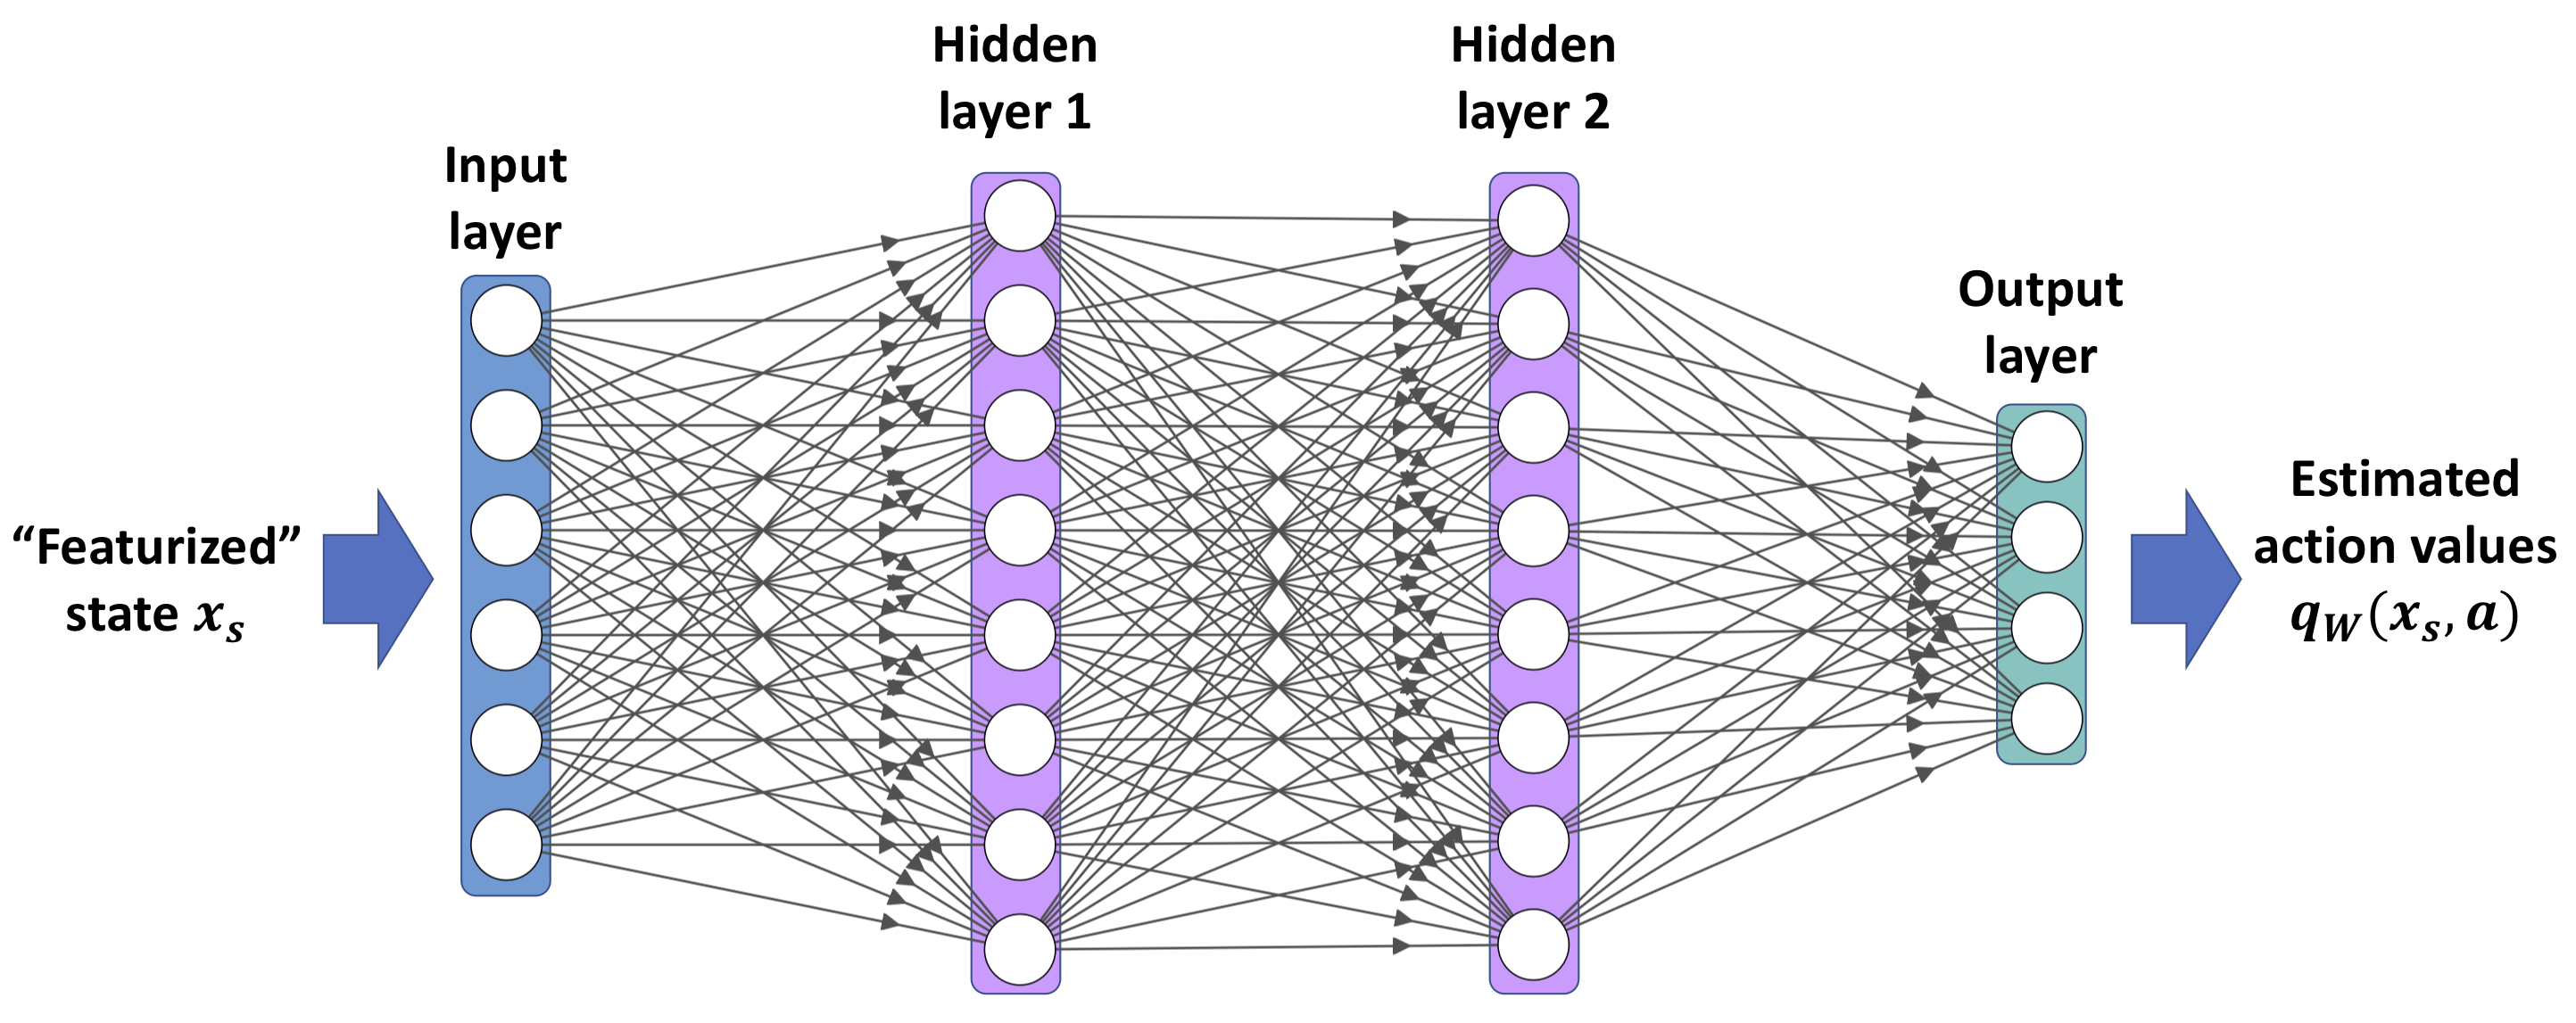
\includegraphics[keepaspectratio, scale=0.55]{images/dqn.png}
		\caption{Exemple de DQN}
	\end{figure}
	
\end{frame}

\begin{frame}{Q-values}
	\frametitle{Q-values}
	
	Pour ce faire, nous pouvons modifier la règle de mise à jour pour prendre en compte la valeur Q maximale en variant les différentes actions dans l'état immédiat suivant. L'équation modifiée pour la mise à jour des valeurs Q est la suivante :
	
	\[
	Q(S_t, A_t) \leftarrow Q(S_t, A_t) + \alpha [R_{t+1} + \gamma \max_{a} Q(S_{t+1}, a) - Q(S_t, A_t)]
	\]
	
\end{frame}


\begin{frame}{Détermination de la valeur cible à l'aide du DQN}
	\frametitle{Détermination de la valeur cible à l'aide du DQN}
	
	\begin{figure}[htpb]
		\centering
		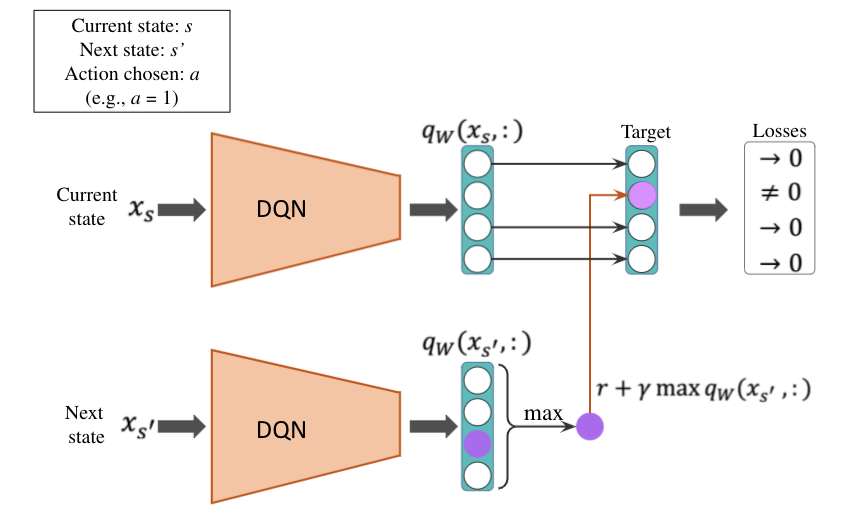
\includegraphics[keepaspectratio, scale=0.3]{images/dqn-target.png}
		\caption{Détermination de la valeur cible à l'aide du DQN}
	\end{figure}
	
\end{frame}


\begin{frame}{Détermination de la valeur cible à l'aide du DQN}
	\frametitle{Détermination de la valeur cible à l'aide du DQN}
	
	Nous traitons cela comme un problème de régression, en utilisant les trois quantités suivantes :
	
	\begin{itemize}
		\item Les valeurs prédites actuellement, \( q_w(x_s, :) \)
		\item Le vecteur de valeur cible tel que décrit
		\item La fonction de perte standard d'erreur quadratique moyenne (MSE)
	\end{itemize}
	
\end{frame}



% --- Thank you slide ---

\begin{frame}
	\begin{center}
		
		\Huge \textbf{Merci pour Votre Attention !}
		
		\vspace{1cm}
		
		\Large
		
		\textit{Abdelhakim Zetati -- Lahcen Ezzara} \\
		

	\end{center}
\end{frame}


\end{document}